\chapter[Tutorial esencial de LaTeX: Fundamentos y Conceptos Clave]{Tutorial esencial de LaTeX: Fundamentos y Conceptos Clave}
\label{cp:latex-tutorial}

{
\parindent0pt

En este capítulo se introduce el entorno de trabajo de \LaTeX, destacando los aspectos básicos que necesitarás para redactar tu tesis. A diferencia de los editores de tipo \textit{Lo que ves es lo que obtienes} como Microsoft Word, \LaTeX utiliza archivos de texto plano que contienen tanto el contenido como los comandos de formato. Estos archivos son procesados por un motor TeX, que interpreta dichos comandos para producir un PDF maquetado con precisión tipográfica.

Este enfoque te permite centrarte en el contenido, dejando la responsabilidad del diseño y la presentación a \LaTeX y al motor TeX, garantizando así un resultado profesional en todo momento. Aunque en este capítulo se presentarán algunas funcionalidades clave, se recomienda encarecidamente aprender \LaTeX desde sus fundamentos. Puedes consultar en cualquier momento la serie de Overleaf \href{https://www.overleaf.com/learn/latex/Learn_LaTeX_in_30_minutes}{Learn LaTeX} como guía de referencia.
}

\section{Citas}
\label{sec:citations}

Existen dos formas principales de citar entradas de la bibliografía. El primer método consiste en instalar un gestor de bibliografías. Existen multiples en el mercado (Mendeley, Zotero, Endnote etc.). Actualmente, la UMU tiene una colaboración con Mendeley (\href{https://www.um.es/web/biblioteca/novedades/-/asset_publisher/XFPBg3QULTgS/content/acceso-a-mendeley-institutional-edition}{(Link)}. Es fácil de usar y se puede sincronizar con Overleaf. 
Una vez hecho esto, para realizar una cita dentro del texto, se utiliza el comando \verb|\cite{ENTRADA}|, y en el mismo comando puedes citar a multiples autores a la vez \verb|\cite{ENTRADA1, ENTRADA2, ENTRADA3}|. 

\begin{block}[tip]
\textit{Citar correctamente es fundamental en la escritura académica, ya que constituye la base de la credibilidad, la transparencia y el avance del conocimiento. Es una práctica esencial de cualquier trabajo académico riguroso. Asegúrate siempre de que tus citas sean precisas y adecuadas.}
\end{block}

\noindent\textbf{Ejemplo:}. Esta plantilla es una modificación de la plantilla IPLeiriaThesis \cite{IPLeiriaThesis}, dando lugar a la creación de UMUthesis \cite{UMU_Thesis}

\section{Referencias}

Al igual que las citas bibliográficas, es altamente recomendable referenciar elementos clave dentro del documento, como capítulos, secciones, figuras o tablas. Para ello, primero debes crear una etiqueta utilizando el comando \verb|\label{TEXTO}|, colocándola dentro del elemento que deseas referenciar. Una vez creada la etiqueta, puedes hacer referencia a ella con \verb|\ref{ETIQUETA}|.

\textbf{Se recomienda encarecidamente utilizar} \verb|\autoref{ETIQUETA}|. Este comando genera un enlace automático con el tipo de elemento correspondiente (por ejemplo, capítulo, sección, figura...), y lo presenta con el formato adecuado. Por ejemplo, una referencia a un capítulo se verá así: \autoref{cp:introduction}, en lugar de simplemente Capítulo \ref{cp:introduction}.

\begin{block}[tip]
\textit{Referenciar correctamente elementos del documento, como \textbf{capítulos, secciones, figuras, tablas o listados}, es fundamental para garantizar la claridad y estructura del texto.}
\end{block}

\section{Glosario y Acrónimos}

Este documento incluye tanto un glosario como una lista de acrónimos, disponibles al inicio del trabajo. Puedes crear una nueva entrada en los archivos ubicados en \verb|Matter/02-Glossary| (para términos) o \verb|Matter/03-Acronyms| (para acrónimos), dependiendo del tipo de concepto que desees añadir.

Una vez añadida la entrada, puedes referenciarla dentro del texto de las siguientes maneras:

- Para entradas del glosario, usa \verb|\gls{ENTRADA}|.
- Para acrónimos, tienes dos opciones:
  - \verb|\acrfull{ENTRADA}|: se utiliza la primera vez que aparece el acrónimo y muestra su significado completo.
  - \verb|\acrshort{ENTRADA}|: para menciones posteriores sin repetir la definición.

\vspace{.875em}
\textbf{Ejemplo:} Utilizar \Gls{latex} para \Gls{maths} es fundamental (...). Es aconsejable obtener tanto el \acrfull{gcd} como el \acrfull{lcm} porque (...). Más adelante, con la ayuda del \acrshort{gcd} y el \acrshort{lcm}, podemos (...).

\section{Figuras}

En \LaTeX, insertar figuras es un proceso sencillo. Para ello, se debe utilizar el entorno \verb|\begin{figure}|. Puedes ajustar el parámetro \verb|width| según tus necesidades, pero es fundamental elegir imágenes de alta calidad para garantizar un buen resultado visual.

También es importante añadir un pie de figura (caption) bien redactado. Si la figura proviene de una fuente externa, considera incluir una cita o referencia. El pie de figura se crea con el comando \verb|\caption{TEXTO}|. Si deseas una versión abreviada del pie de figura para que aparezca en la Tabla de Figuras, usa el formato \verb|\caption[TEXTO_CORTO]{TEXTO_COMPLETO}|.

Siguiendo estas recomendaciones, podemos generar una figura como se muestra en la \autoref{fig:figure-01}.

\begin{figure}[!htpb]
    \centering
    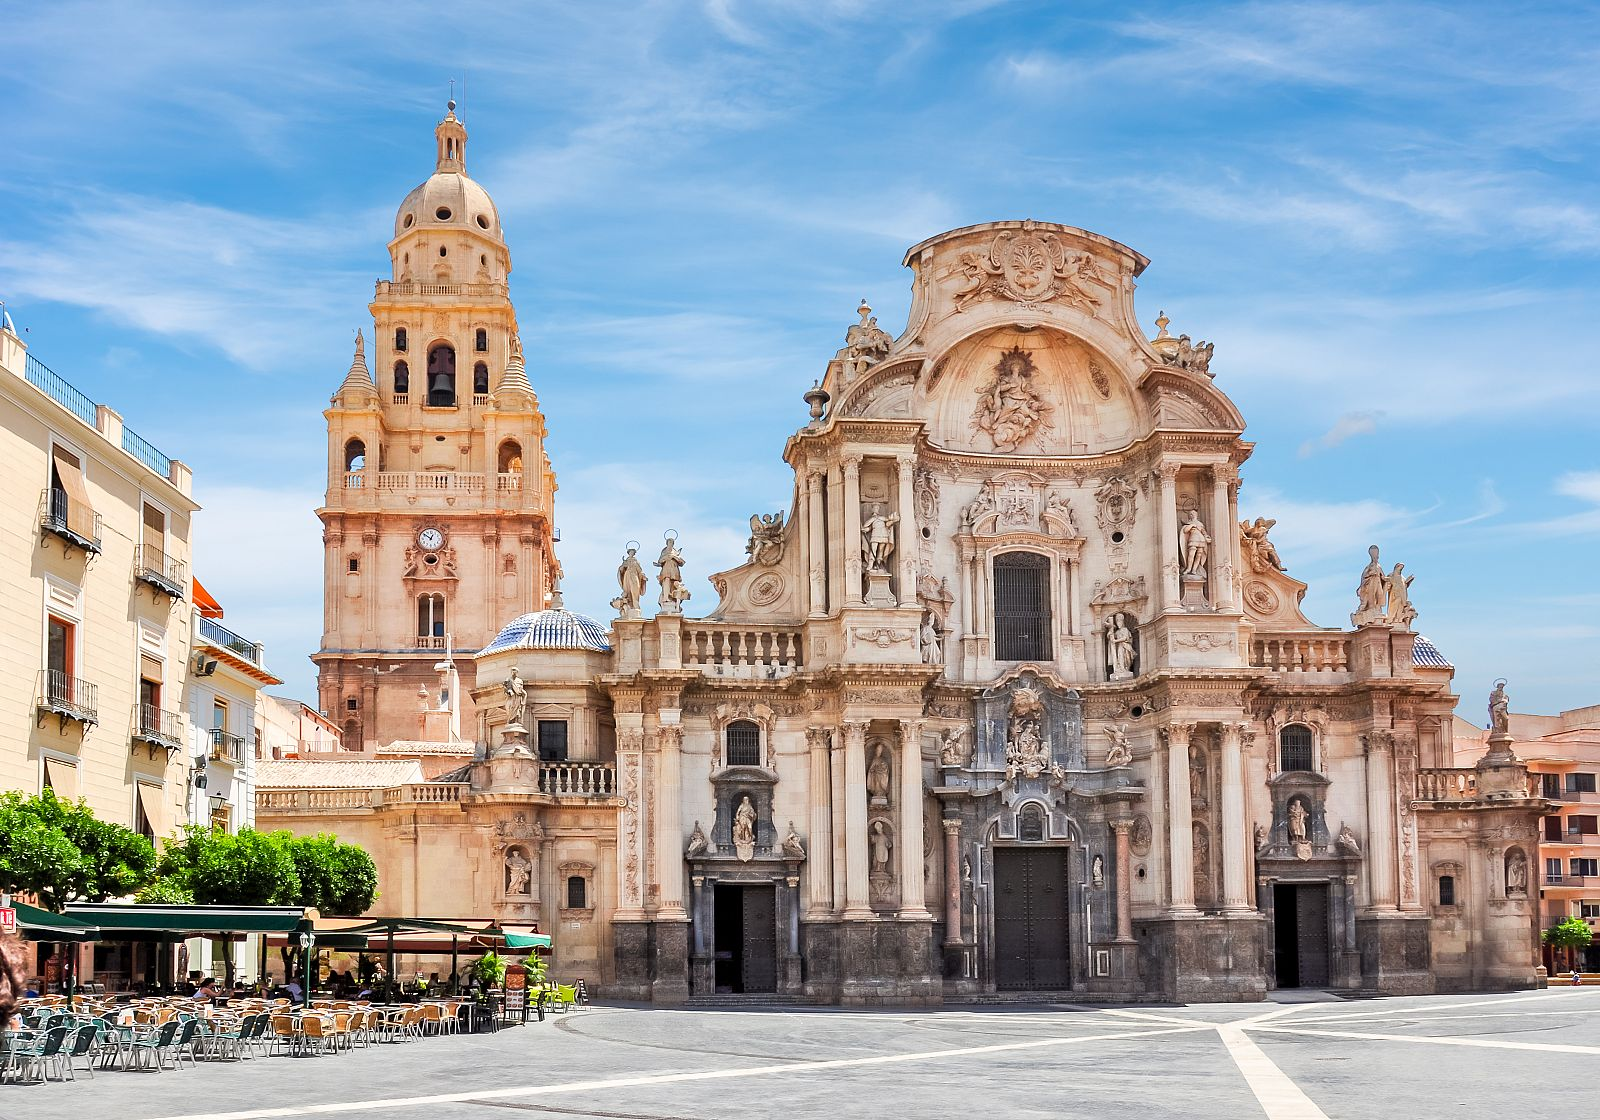
\includegraphics[width=\linewidth]{Figures/catedral.jpg}
    \caption[La catedral más bonita del mundo]{Ilustración de la catedrál más bonita del mundo).}
    \label{fig:figure-01}
\end{figure}

Si deseas comparar imágenes u organizarlas una al lado de la otra, puedes utilizar los entornos \verb|\begin{figure}| y \verb|\begin{subfigure}| de forma conjunta. Luego, puedes referenciar las subfiguras como \autoref{fig:figure-02.1} y \autoref{fig:figure-02.2}.

\begin{figure}[!htpb]
    \centering
    \begin{subfigure}{0.45\textwidth}
        \centering
        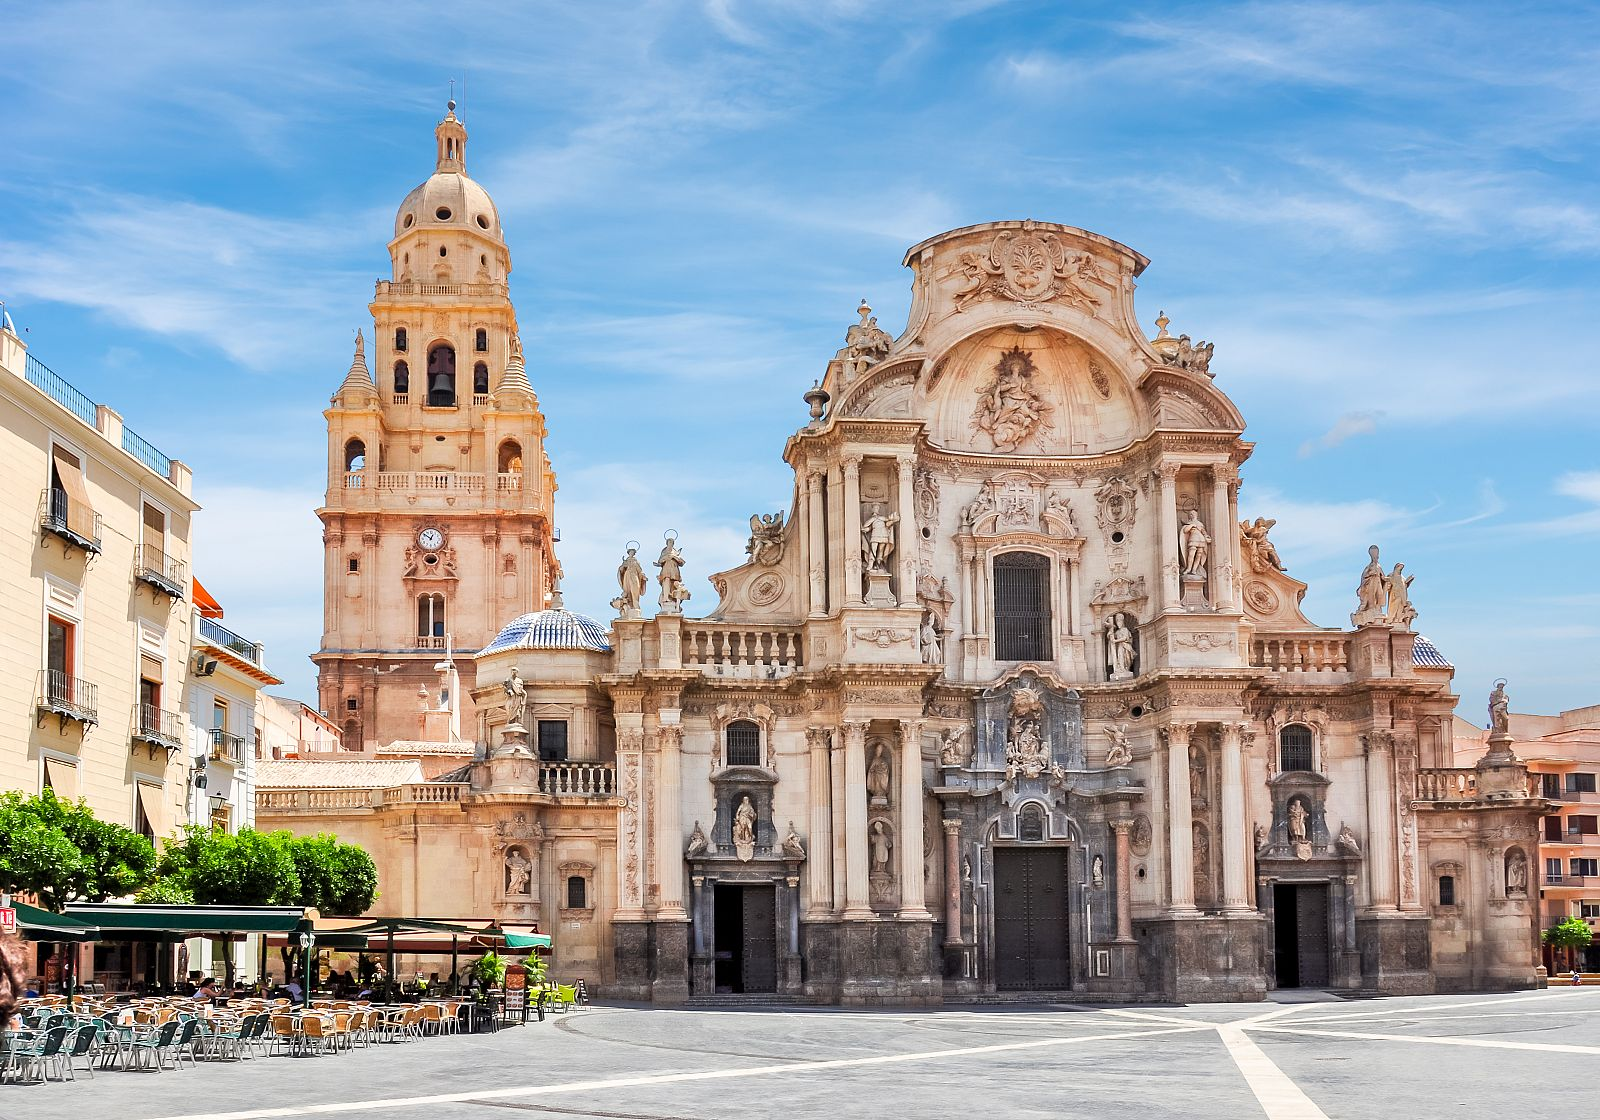
\includegraphics[width=0.9\textwidth]{Figures/catedral.jpg}
        \caption{Subfigura 1.}
        \label{fig:figure-02.1}
    \end{subfigure}
    \hspace{.5cm}
    \begin{subfigure}{0.45\textwidth}
        \centering
        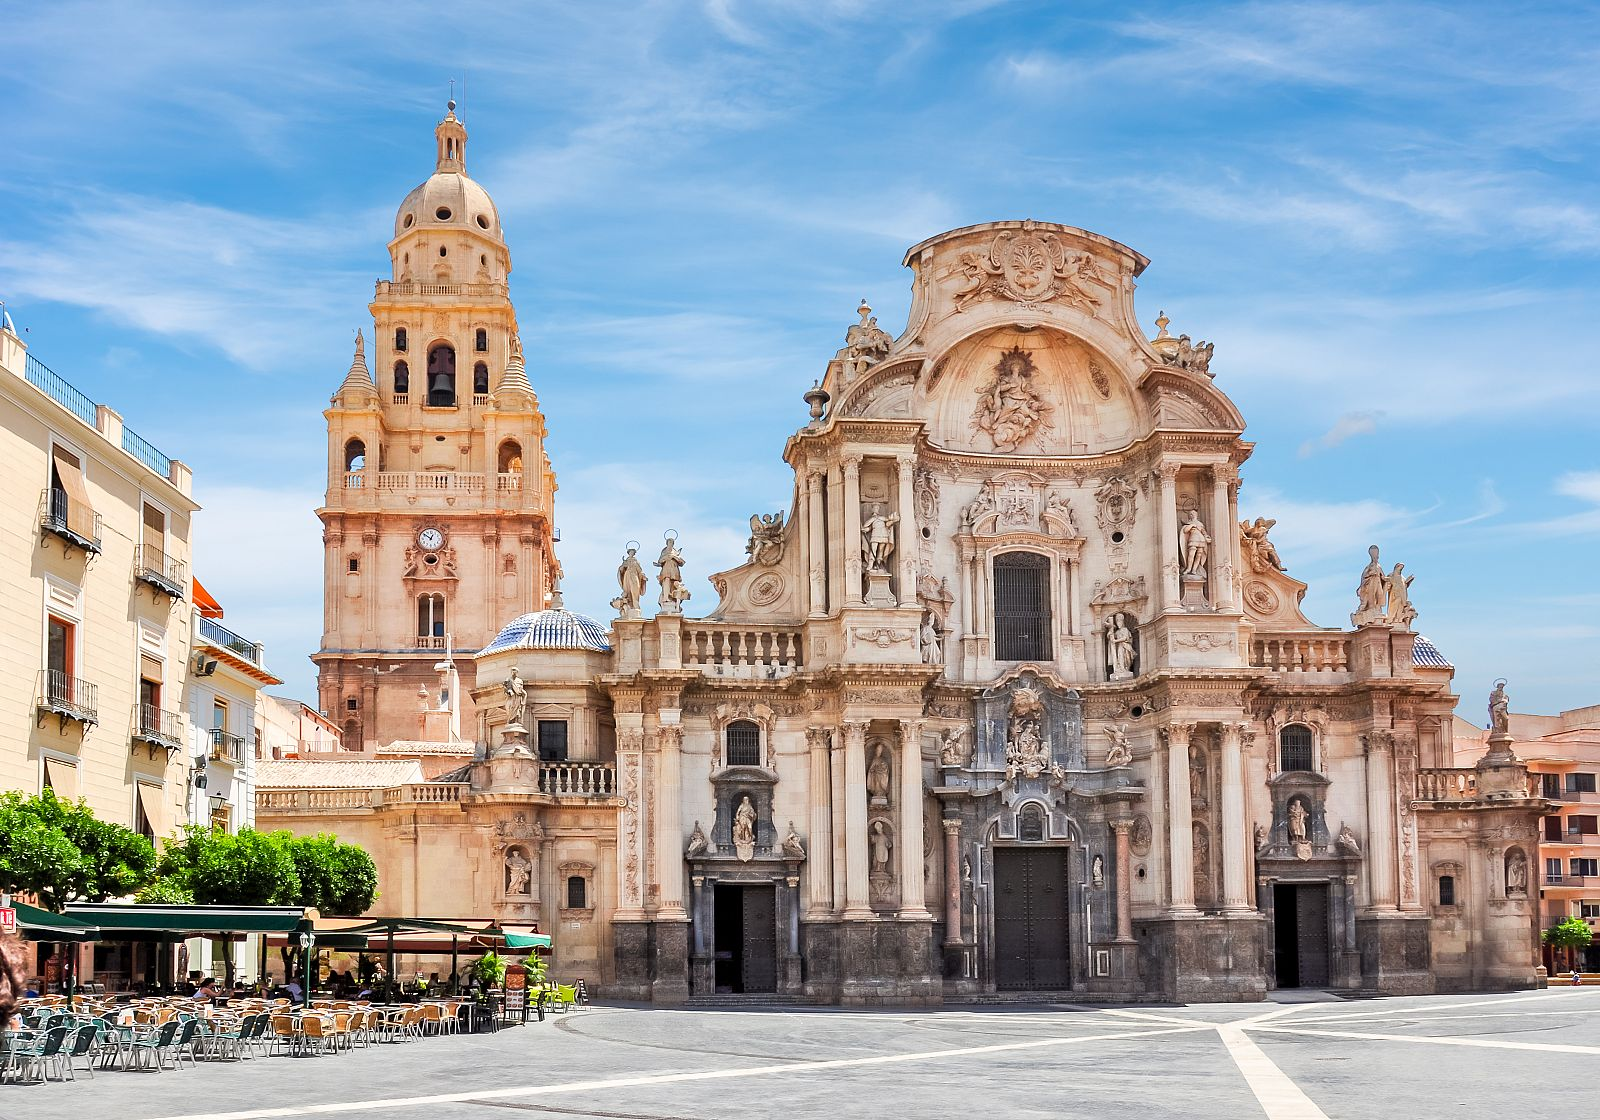
\includegraphics[width=0.9\textwidth]{Figures/catedral.jpg}
        \caption{Subfigura 2.}
        \label{fig:figure-02.2}
    \end{subfigure}
    \caption{La catedral más bonita del mundo.}
    \label{fig:figure-02}
\end{figure}

\section{Tablas}

Las tablas son esenciales para presentar resultados e información de forma clara. En esta sección se presentan distintas técnicas para mostrar datos utilizando los entornos disponibles en esta plantilla. Aunque definir tablas en \LaTeX pueda parecer complicado al principio, esta plantilla simplifica considerablemente el proceso.

\begin{block}[tip]
\textit{Antes de mostrar los diferentes entornos de tablas, es importante recordar que todas deben estar dentro del entorno \texttt{\textbackslash begin\{table\}}. Además, se recomienda utilizar la opción de flotación \texttt{[!htpb]} para mejorar la colocación automática de las tablas en el documento. \textbf{Este consejo también aplica al uso de figuras.}}
\end{block}

\subsection{Entorno Tabular}

El entorno estándar \verb|\begin{tabular}| permite crear tablas simples pero elegantes. La tabla \autoref{tab:table-01} se ha generado utilizando un entorno centrado (\verb|\centering|) y empleando el paquete \verb|booktabs| para mejorar el estilo visual.

\begin{table}[!htpb]
    \caption{Ejemplo de uso del entorno tabular.}
    \label{tab:table-01}
    \centering
    \begin{tabular}{llc}
        \toprule
        \textbf{Encabezado 1} & \textbf{Encabezado 2} & \textbf{Encabezado 3} \\
        \midrule
        Lorem Ipsum         & Pharetra Dolor    & $\checkmark$  \\
        Amet Consectetuer   & Curabitur Aliquet & -             \\
        Praesent Mauris     & Praesent Libero   & $\checkmark$  \\
        \bottomrule
    \end{tabular}
\end{table}


\subsection{Entorno Tabularx}

El paquete \verb|tabularx| permite construir tablas con columnas que se expanden automáticamente para ocupar todo el ancho disponible. Para lograr este comportamiento, se puede utilizar el entorno: \verb|\begin{tabularx}{\textwidth}{lX}|, donde la columna \verb|X| se comporta como una columna multicolumna que ocupa el espacio restante. La tabla \autoref{tab:table-02} muestra un ejemplo del uso de este entorno.

\begin{table}[!htpb]
    \caption{Ejemplo del uso del entorno tabularx.}
    \label{tab:table-02}
    \begin{tabularx}{\textwidth}{lX}
        \toprule
        \textbf{Encabezado 1} & \textbf{Encabezado 2} \\ 
        \midrule
        Foo Bar Baz & Quisque cursus, metus vitae pharetra auctor, sem massa mattis sem, at interdum magna augue eget diam. \\
        Ipsum Dolor & Vestibulum ante ipsum primis in faucibus orci luctus et ultrices posuere cubilia Curae; Curabitur aliquet quam id dui. \\
        Dolor Sit & Phasellus condimentum elementum justo, quis interdum est sagittis ac. Vestibulum non arcu sit amet justo lobortis semper. \\
        Amet Consectetuer & Integer nec odio praesent libero sed cursus ante dapibus diam sed nisi vestibulum non arcu. \\
        Consectetuer Adipiscing & Nulla quis sem at nibh elementum imperdiet. Duis sagittis ipsum. Praesent mauris. \\
        \bottomrule
    \end{tabularx}
\end{table}

\subsection{Entorno Longtable}

Cuando se trabaja con tablas especialmente largas que necesitan dividirse en varias páginas, es conveniente usar el entorno \verb|\begin{longtable}|. Este entorno requiere definir el encabezado dos veces: una para la primera aparición de la tabla y otra para las siguientes páginas. Esto garantiza que el lector pueda identificar correctamente las columnas en todo momento. Consulta la \autoref{tab:table-03} para ver un ejemplo detallado.

\begin{longtable}[c]{lll}
\caption{Ejemplo del uso del entorno longtable.}
\label{tab:table-03} \\
\toprule
\textbf{Nombre} & \textbf{Correo electrónico} & \textbf{Rol o puesto} \\ 
\midrule
\endfirsthead

\multicolumn{3}{c}%
{{\textit{\bfseries Tabla \thetable\ continuación de la página anterior.}}} \\
\toprule
\textbf{Nombre} & \textbf{Correo electrónico} & \textbf{Rol o puesto} \\ 
\midrule
\endhead

\bottomrule
\addlinespace[1mm]
\multicolumn{3}{r}%
{{\textit{Continúa en la siguiente página.}}} \\
\endfoot
\bottomrule
\endlastfoot

Alice Johnson & alice.johnson@email.com & Project Manager \\
Bob Thompson & bob.thompson@email.com & Data Analyst \\
Charlie Davis & charlie.davis@email.com & Marketing Specialist \\
% (continúa con el resto de la tabla...)
Steven Martin & steven.martin@email.com & Robotics Engineer \\
\end{longtable}

\subsection{Tablas Complejas}

Crear tablas complejas en \LaTeX puede ser una tarea algo desafiante. Por ello, se recomienda encarecidamente el uso de herramientas como \href{https://www.tablesgenerator.com/}{Table Generator}. Esta herramienta permite diseñar visualmente la tabla con el estilo deseado y luego copiar fácilmente el código generado al documento LaTeX. 

Este enfoque simplifica el proceso y asegura una representación precisa del contenido. No obstante, es fundamental que la tabla siga siendo comprensible para el lector. \textbf{El exceso de complejidad puede dificultar la interpretación}. La \autoref{tab:table-04} muestra un ejemplo de tabla con múltiples niveles de detalle.

\begin{table}[!htpb]
    \caption{Ejemplo del uso de tablas complejas.}
    \label{tab:table-04}
    \centering
    \begin{tabular}{lcc}
        \toprule
        \multirow{2}{*}{\textbf{Componente}} & \multicolumn{2}{c}{\textbf{Especificaciones}} \\
        \cmidrule(lr){2-3}
        & \textbf{Característica} & \textbf{Compatible} \\
        \midrule
        \multirow{4}{*}{CPU} & Núcleos (ej.: 8) & $\checkmark$ \\
        & Frecuencia base (ej.: 3.6 GHz) & $\checkmark$ \\
        & Hyper-Threading & $\checkmark$ \\
        & Gráficos integrados & - \\
        \midrule
        \multirow{4}{*}{GPU} & Núcleos CUDA (ej.: 5120) & $\checkmark$ \\
        & Frecuencia base (ej.: 1.5 GHz) & $\checkmark$ \\
        & Soporte Ray Tracing & $\checkmark$ \\
        & Multi-GPU (SLI/CrossFire) & - \\
        \midrule
        \multirow{4}{*}{Memoria} & Tipo (ej.: DDR5, GDDR6) & $\checkmark$ \\
        & Capacidad (ej.: 16 GB) & $\checkmark$ \\
        & Ancho de banda (ej.: 448 GB/s) & $\checkmark$ \\
        & Soporte ECC & - \\
        \midrule
        \multirow{3}{*}{Placa Base} & Soporte PCIe 5.0 & $\checkmark$ \\
        & Wi-Fi 6E & $\checkmark$ \\
        & Thunderbolt 4 & - \\
        \bottomrule
    \end{tabular}
\end{table}

\section{Listas}

Crear listas en \LaTeX es sencillo y ofrece varias opciones según tus necesidades. Puedes generar listas con viñetas mediante el entorno \verb|\begin{itemize}| o listas numeradas con \verb|\begin{enumerate}|. A continuación se muestra un ejemplo con el entorno \verb|itemize|:

\begin{itemize}
  \item Cada elemento comienza con el comando \verb|\item|.
  \item Los elementos están marcados con un punto negro (viñeta).
  \item El texto de cada elemento puede tener cualquier longitud.
\end{itemize}

Como se mencionó anteriormente, también puedes crear una lista numerada con el entorno \verb|enumerate|. Por ejemplo:

\begin{enumerate}
  \item Los elementos se numeran automáticamente.
  \item La numeración comienza en 1 en cada entorno \verb|enumerate|.
  \item Otro elemento más en la lista.
\end{enumerate}

También es posible anidar listas dentro de otras listas del mismo tipo. Aquí tienes un ejemplo:

\begin{enumerate}
    \item Elemento de primer nivel
    \item Elemento de primer nivel
    \begin{enumerate}
        \item Elemento de segundo nivel
        \item Elemento de segundo nivel
        \begin{enumerate}
            \item Elemento de tercer nivel
            \item Elemento de tercer nivel
        \end{enumerate}
    \end{enumerate}
\end{enumerate}

\begin{block}[tip]
\textit{Observa que las etiquetas cambian automáticamente según el nivel, aunque se use el mismo entorno para todas las listas. \textbf{Esto demuestra que no es necesario cambiar de entorno para lograr una numeración jerárquica.}}
\end{block}

También puedes personalizar la etiqueta de cada ítem según tus necesidades. Para ello, basta con añadir un nuevo \verb|\item| y colocar la etiqueta deseada entre corchetes. Por ejemplo, \verb|\item[!]| mostrará un signo de exclamación como viñeta. A continuación se muestran algunos ejemplos:

\begin{itemize}
  \item Este es mi primer punto
  \item Otro punto que quiero destacar
  \item[!] ¡Un punto importante!
  \item[$\blacksquare$] Un punto fuerte y cuadrado
  \item[] ¿Una etiqueta vacía?
\end{itemize}

Por último, puedes utilizar una lista descriptiva. A diferencia de las listas con viñetas o numeradas, este tipo permite asignar una descripción personalizada a cada elemento. En el siguiente ejemplo, hay tres entradas: dos con descripción y una sin etiqueta:

\begin{description}
    \item[Elemento 1:] Este es el primer ítem con descripción.
    \item[Elemento 2:] Otro ítem con una descripción diferente.
    \item Un ítem sin una etiqueta específica.
\end{description}

\section{Listados de Código}

A veces puede ser útil incluir fragmentos de código fuente directamente en tu documento. Para ello, puedes usar dos entornos anidados: \verb|\begin{listing}|, que permite añadir título y etiqueta, y \verb|\begin{minted}|, que aplica resaltado de sintaxis.

\autoref{listing:c-code} muestra un ejemplo de código en lenguaje C:

\begin{listing}[!htpb]
\caption{Hola mundo en C.}
\label{listing:c-code}
\begin{minted}{c}
#include <stdio.h>
int main() {
   printf("Hello, World!"); /* printf() imprime la cadena */
   return 0;
}
\end{minted}
\end{listing}

El código anterior está incluido directamente en el documento. Sin embargo, también puedes importar código desde un archivo externo. Para ello, utiliza el comando \verb|\inputminted{LENGUAJE}{ARCHIVO}| dentro del entorno \verb|listing|. En el siguiente ejemplo, se importa código Haskell:

\begin{listing}[!htpb]
\caption{Factorial en Haskell.}
\label{listing:haskell-code}
\inputminted{haskell}{Code/Factorial.hs}
\end{listing}

En algunos casos, cuando solo necesitas resaltar un comando específico, no es necesario usar \verb|listing| ni \verb|minted|. Puedes usar el comando \verb|\verb| para resaltar texto en línea o \verb|\begin{verbatim}| para bloques largos.

Ejemplo:

\begin{verbatim}
\begin{listing}[!htpb]
    \inputminted{LENGUAJE}{ARCHIVO}
    \caption{TÍTULO}
    \label{ETIQUETA}
\end{listing}
\end{verbatim}

Si el fragmento de código es demasiado largo y ocupa varias páginas, puedes usar el entorno \verb|\begin{longlisting}|, que divide automáticamente el contenido en varias páginas. Un ejemplo se muestra en \autoref{listing:lisp-code}.

\begin{longlisting}
\caption{Ejemplo de funciones en Lisp.}
\label{listing:lisp-code}
\begin{minted}{lisp}
(defun factorial (n)
  "Calcula el factorial de un número."
  (if (zerop n)
      (* n (factorial (1- n)))))

(defun fibonacci (n)
  "Calcula el n-ésimo número de Fibonacci."
  (cond ((zerop n) 0)
        ((= n 1) 1)
        (t (+ (fibonacci (1- n)) (fibonacci (- n 2))))))

(defun gcd (a b)
  "Calcula el máximo común divisor entre a y b."
  (if (zerop b)
      a
      (gcd b (mod a b))))

(defun primes-up-to (limit)
  "Devuelve una lista de todos los números primos hasta LIMIT."
  (let ((primes '()))
    (loop for i from 2 to limit
          unless (some (lambda (p) (zerop (mod i p))) primes)
          do (push i primes))
    (nreverse primes)))

(defun example-function (x)
  "Función de ejemplo para demostrar capacidades en Lisp."
  (let ((result (list (factorial x)
                      (fibonacci x)
                      (gcd x 10)
                      (primes-up-to x))))
    (format t "Factorial de ~A: ~A~%" x (factorial x))
    (format t "Fibonacci de ~A: ~A~%" x (fibonacci x))
    (format t "MCD de ~A y 10: ~A~%" x (gcd x 10))
    (format t "Primos hasta ~A: ~A~%" x (primes-up-to x))
    result))

(example-function 10)
\end{minted}
\end{longlisting}

\section{Ecuaciones}

Al redactar ecuaciones o expresiones matemáticas, \LaTeX es una herramienta potente y versátil. Puedes introducir fórmulas en modo en línea usando el entorno \verb|\(FORMULA\)| o utilizar \verb|\begin{equation}| para mostrar la ecuación en modo matemático con numeración. Si prefieres que la ecuación no tenga numeración, puedes usar el entorno \verb|\[FORMULA\]|.

\vspace{.875em}
\textbf{Ejemplo:} En física, la equivalencia entre masa y energía se expresa mediante la ecuación \(E=mc^2\), descubierta en 1905 por Albert Einstein. En unidades naturales ($c = 1$), la fórmula (\ref{eq:equation-01}) expresa la siguiente identidad:

\begin{equation}
\label{eq:equation-01}
E = m.c^2
\end{equation}

\textbf{Ejemplo:} A continuación se muestra una ecuación —\textit{sin numeración}— que representa una función de pérdida regularizada en aprendizaje supervisado, combinando la pérdida media de predicción sobre el conjunto de entrenamiento y un término de regularización $L_2$ para evitar el sobreajuste:

\[
\mathcal{L}(\boldsymbol{\theta}) = \frac{1}{N} \sum_{i=1}^{N} \ell(y_i, f(\mathbf{x}_i; \boldsymbol{\theta})) + \lambda \|\boldsymbol{\theta}\|_2^2
\]

Crear ecuaciones puede resultar complejo, por lo que recomendamos usar un editor en línea como \href{https://latexeditor.lagrida.com/}{LaTeX Equation Editor}. Solo tienes que construir la fórmula, copiarla y pegarla en tu documento, ya sea en línea o en un bloque matemático.

\section{Notas al pie}

En ocasiones, puede ser útil presentar información complementaria que no forma parte del cuerpo principal del texto. En \LaTeX, esto se puede hacer fácilmente usando el comando \verb|\footnote{TEXTO}|. El contenido aparecerá al pie de la página\footnote{Esto es una nota.}.

Si deseas insertar notas al pie dentro de una tabla, es mejor replantearlo, ya que \LaTeX no ofrece una forma sencilla de manejarlas. En su lugar, puedes colocar un asterisco “*” donde quieras que aparezca la referencia. Luego, debajo de la tabla —\textbf{pero antes de cerrar el entorno \texttt{table}}— coloca el texto asociado al asterisco. Así lograrás un efecto similar al de una nota al pie, pero localizada bajo la tabla y no al final de la página.
